


\section{Previous Results}

As mentioned previously, this thesis is a continuation of a project done over the previous year in
which we developed a method to use pulsar timing data to constrain our mass models of the globular
cluster 47\,Tuc. The final results of that project were a set of models that accurately reproduce
all observables and fully incorporated the pulsar data in the likelihood. Figure
\ref{fig:nobin_obs_panel} shows the model fits to most of the observables while Figure
\ref{fig:nobin_mass_fun} shows the fit to the stellar mass function data. In both cases, the model
satisfyingly reproduces all observables. The median and $1\sigma$ credibility intervals of the
best-fit parameters are listed in Table \ref{tab:parameters_nobin}.

One of the most interesting results of the previous project was the model's ability to constrain the
black hole content within 47\,Tuc. Figure \ref{fig:prev_nobin_BH_dists} shows the distribution of
mass in black hole mass and number of black holes in our set of best-fit models, which were found to
be $135^{+104}_{-92} \ \mathrm{M}_\odot$ and $26^{+15}_{-15}$ black holes respectively. Both the
total mass and number are quite well contained especially in comparison to the previous constraints
in the literature \citep[see e.g.][]{Henault-Brunet2020,Weatherford2019}.




\begin{table}
	\centering
	\caption{Best-fit parameters with $1\sigma$ credibility intervals for models with a binary fraction of $0\%$.}
	\begin{tabular}{l l}

		\hline
		Parameter                 & Value                  \\
		\hline
		$W_0$                     & $6.26^{+0.11}_{-0.10}$ \\
		$M/10^6 \mathrm{M}_\odot$ & $0.88^{+0.01}_{-0.01}$ \\
		$r_h / pc$                & $6.73^{+0.06}_{-0.06}$ \\
		$\log_{10}{r_a / pc}$     & $1.50^{+0.07}_{-0.05}$ \\
		$g$                       & $1.37^{+0.06}_{-0.06}$ \\
		$\delta$                  & $0.43^{+0.02}_{-0.02}$ \\
		$s^2$                     & $0.01^{+0.01}_{-0.00}$ \\
		$F$                       & $3.25^{+0.14}_{-0.12}$ \\
		$\alpha_1$                & $0.35^{+0.02}_{-0.02}$ \\
		$\alpha_2$                & $1.46^{+0.05}_{-0.05}$ \\
		$\alpha_3$                & $2.13^{+0.04}_{-0.04}$ \\
		$BH_{ret} (\%)$           & $0.07^{+0.06}_{-0.04}$ \\
		$d$                       & $4.42^{+0.02}_{-0.02}$ \\
		\hline
	\end{tabular}
	\label{tab:parameters_nobin}
\end{table}

\begin{figure}
	\centering
	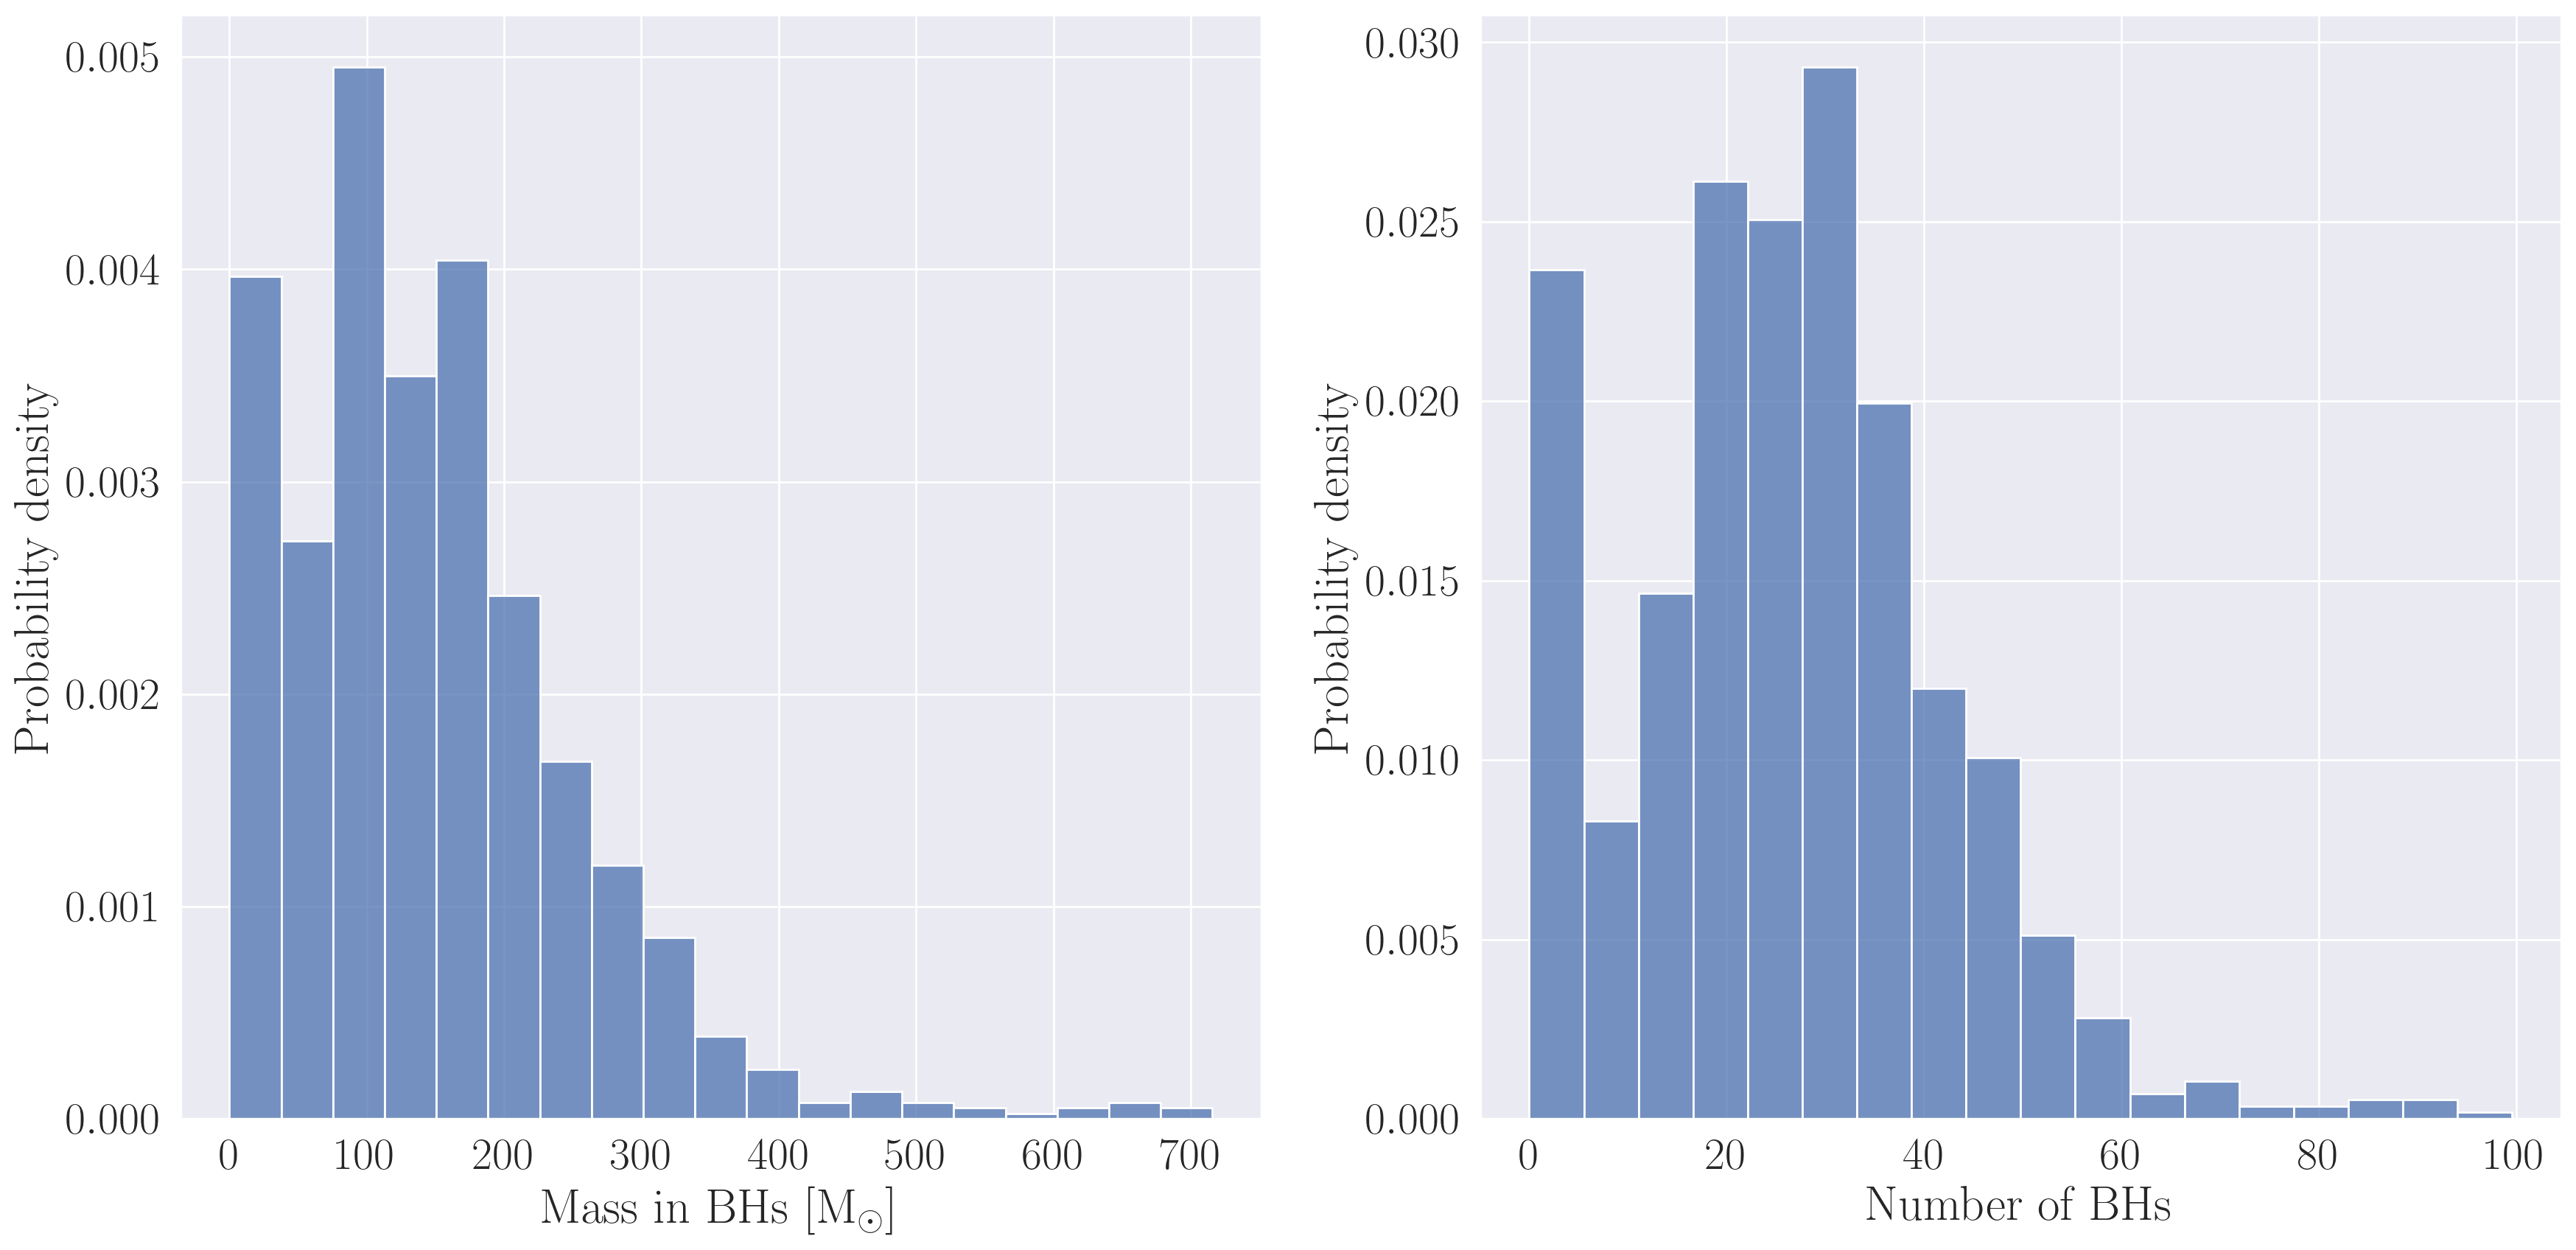
\includegraphics[width=0.8\textwidth]{figures/prev_nobin/BH_dists.png}
	\caption{Distribution in mass and number of black holes for models with a $0\%$ binary
		fraction.}
	\label{fig:prev_nobin_BH_dists}
\end{figure}


\section{Low Binary Fraction}

In the models with a $2\%$ binary fraction, we find a similar ability to reproduce all the
observables, Figure \ref{fig:low_bin_model_obs_panel} and Figure \ref{fig:low_bin_model_mass_fun}
show the model fits compared to the data.

The black hole content in these models is also quite well contained, though different from the
models without binaries. Figure \ref{fig:low_bin_model_BH_dists} shows the distribution of mass in
black holes and number of black holes which this time, are found to be $22^{+13}_{-19}$ black holes or
$114^{+144}_{-79} \mathrm{M}_\odot$ in black holes. The best-fit parameters and the $1\sigma$ credibility
intervals for this set of models are listed in Table \ref{tab:parameters_lowbin}.


\begin{table}
	\centering
	\caption{Best-fit parameters with $1\sigma$ credibility intervals for models with a $2\%$ binary fraction.}
	\begin{tabular}{l l}

		\hline
		Parameter                 & Value                  \\
		\hline
		$W_0$                     & $6.28^{+0.10}_{-0.10}$ \\
		$M/10^6 \mathrm{M}_\odot$ & $0.89^{+0.01}_{-0.01}$ \\
		$r_h / pc$                & $6.74^{+0.06}_{-0.06}$ \\
		$\log_{10}{r_a / pc}$     & $1.50^{+0.06}_{-0.05}$ \\
		$g$                       & $1.36^{+0.06}_{-0.06}$ \\
		$\delta$                  & $0.43^{+0.02}_{-0.02}$ \\
		$s^2$                     & $0.01^{+0.01}_{-0.00}$ \\
		$F$                       & $3.24^{+0.13}_{-0.12}$ \\
		$\alpha_1$                & $0.37^{+0.02}_{-0.02}$ \\
		$\alpha_2$                & $1.47^{+0.05}_{-0.05}$ \\
		$\alpha_3$                & $2.18^{+0.04}_{-0.04}$ \\
		$BH_{ret} (\%)$           & $0.08^{+0.09}_{-0.05}$ \\
		$d$                       & $4.42^{+0.02}_{-0.02}$ \\
		\hline
	\end{tabular}
	\label{tab:parameters_lowbin}
\end{table}

\begin{figure}
	\centering
	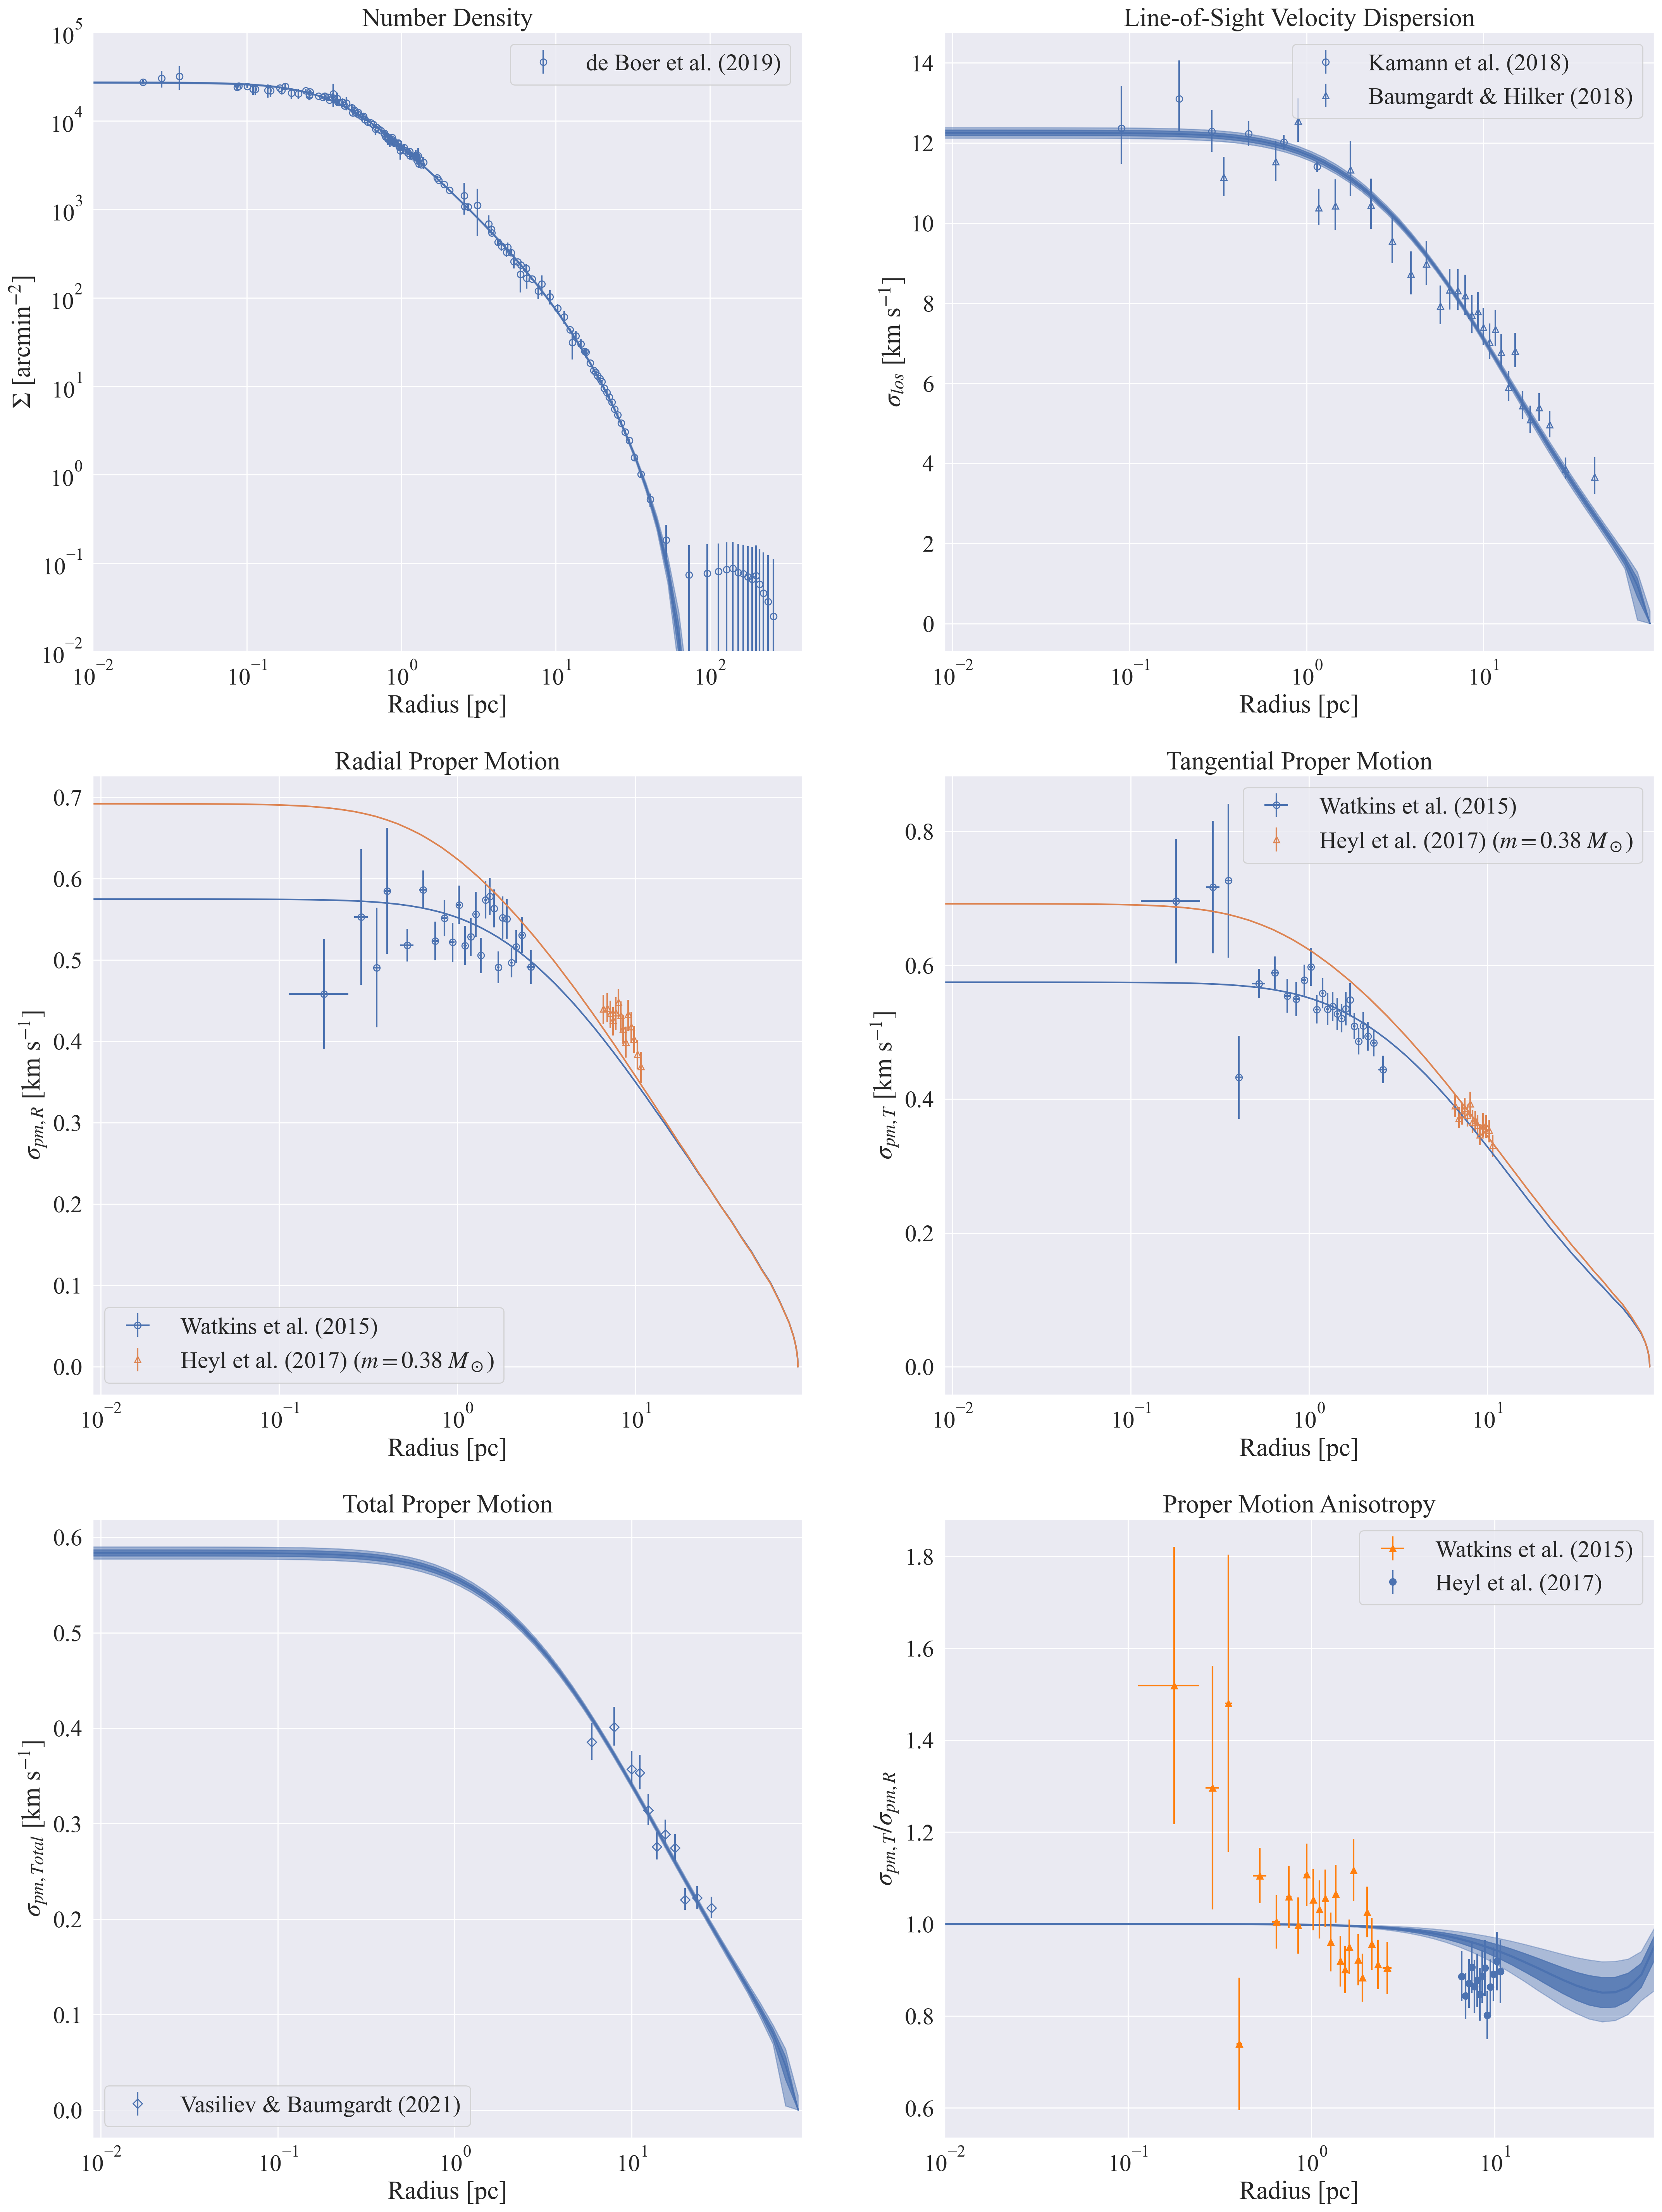
\includegraphics[width=0.9\textwidth]{figures/low_bin_model/obs_panel.png}
	\caption{Model fits to observables for models with a $2\%$ binary fraction.}
	\label{fig:low_bin_model_obs_panel}
\end{figure}


\begin{figure}
	\centering
	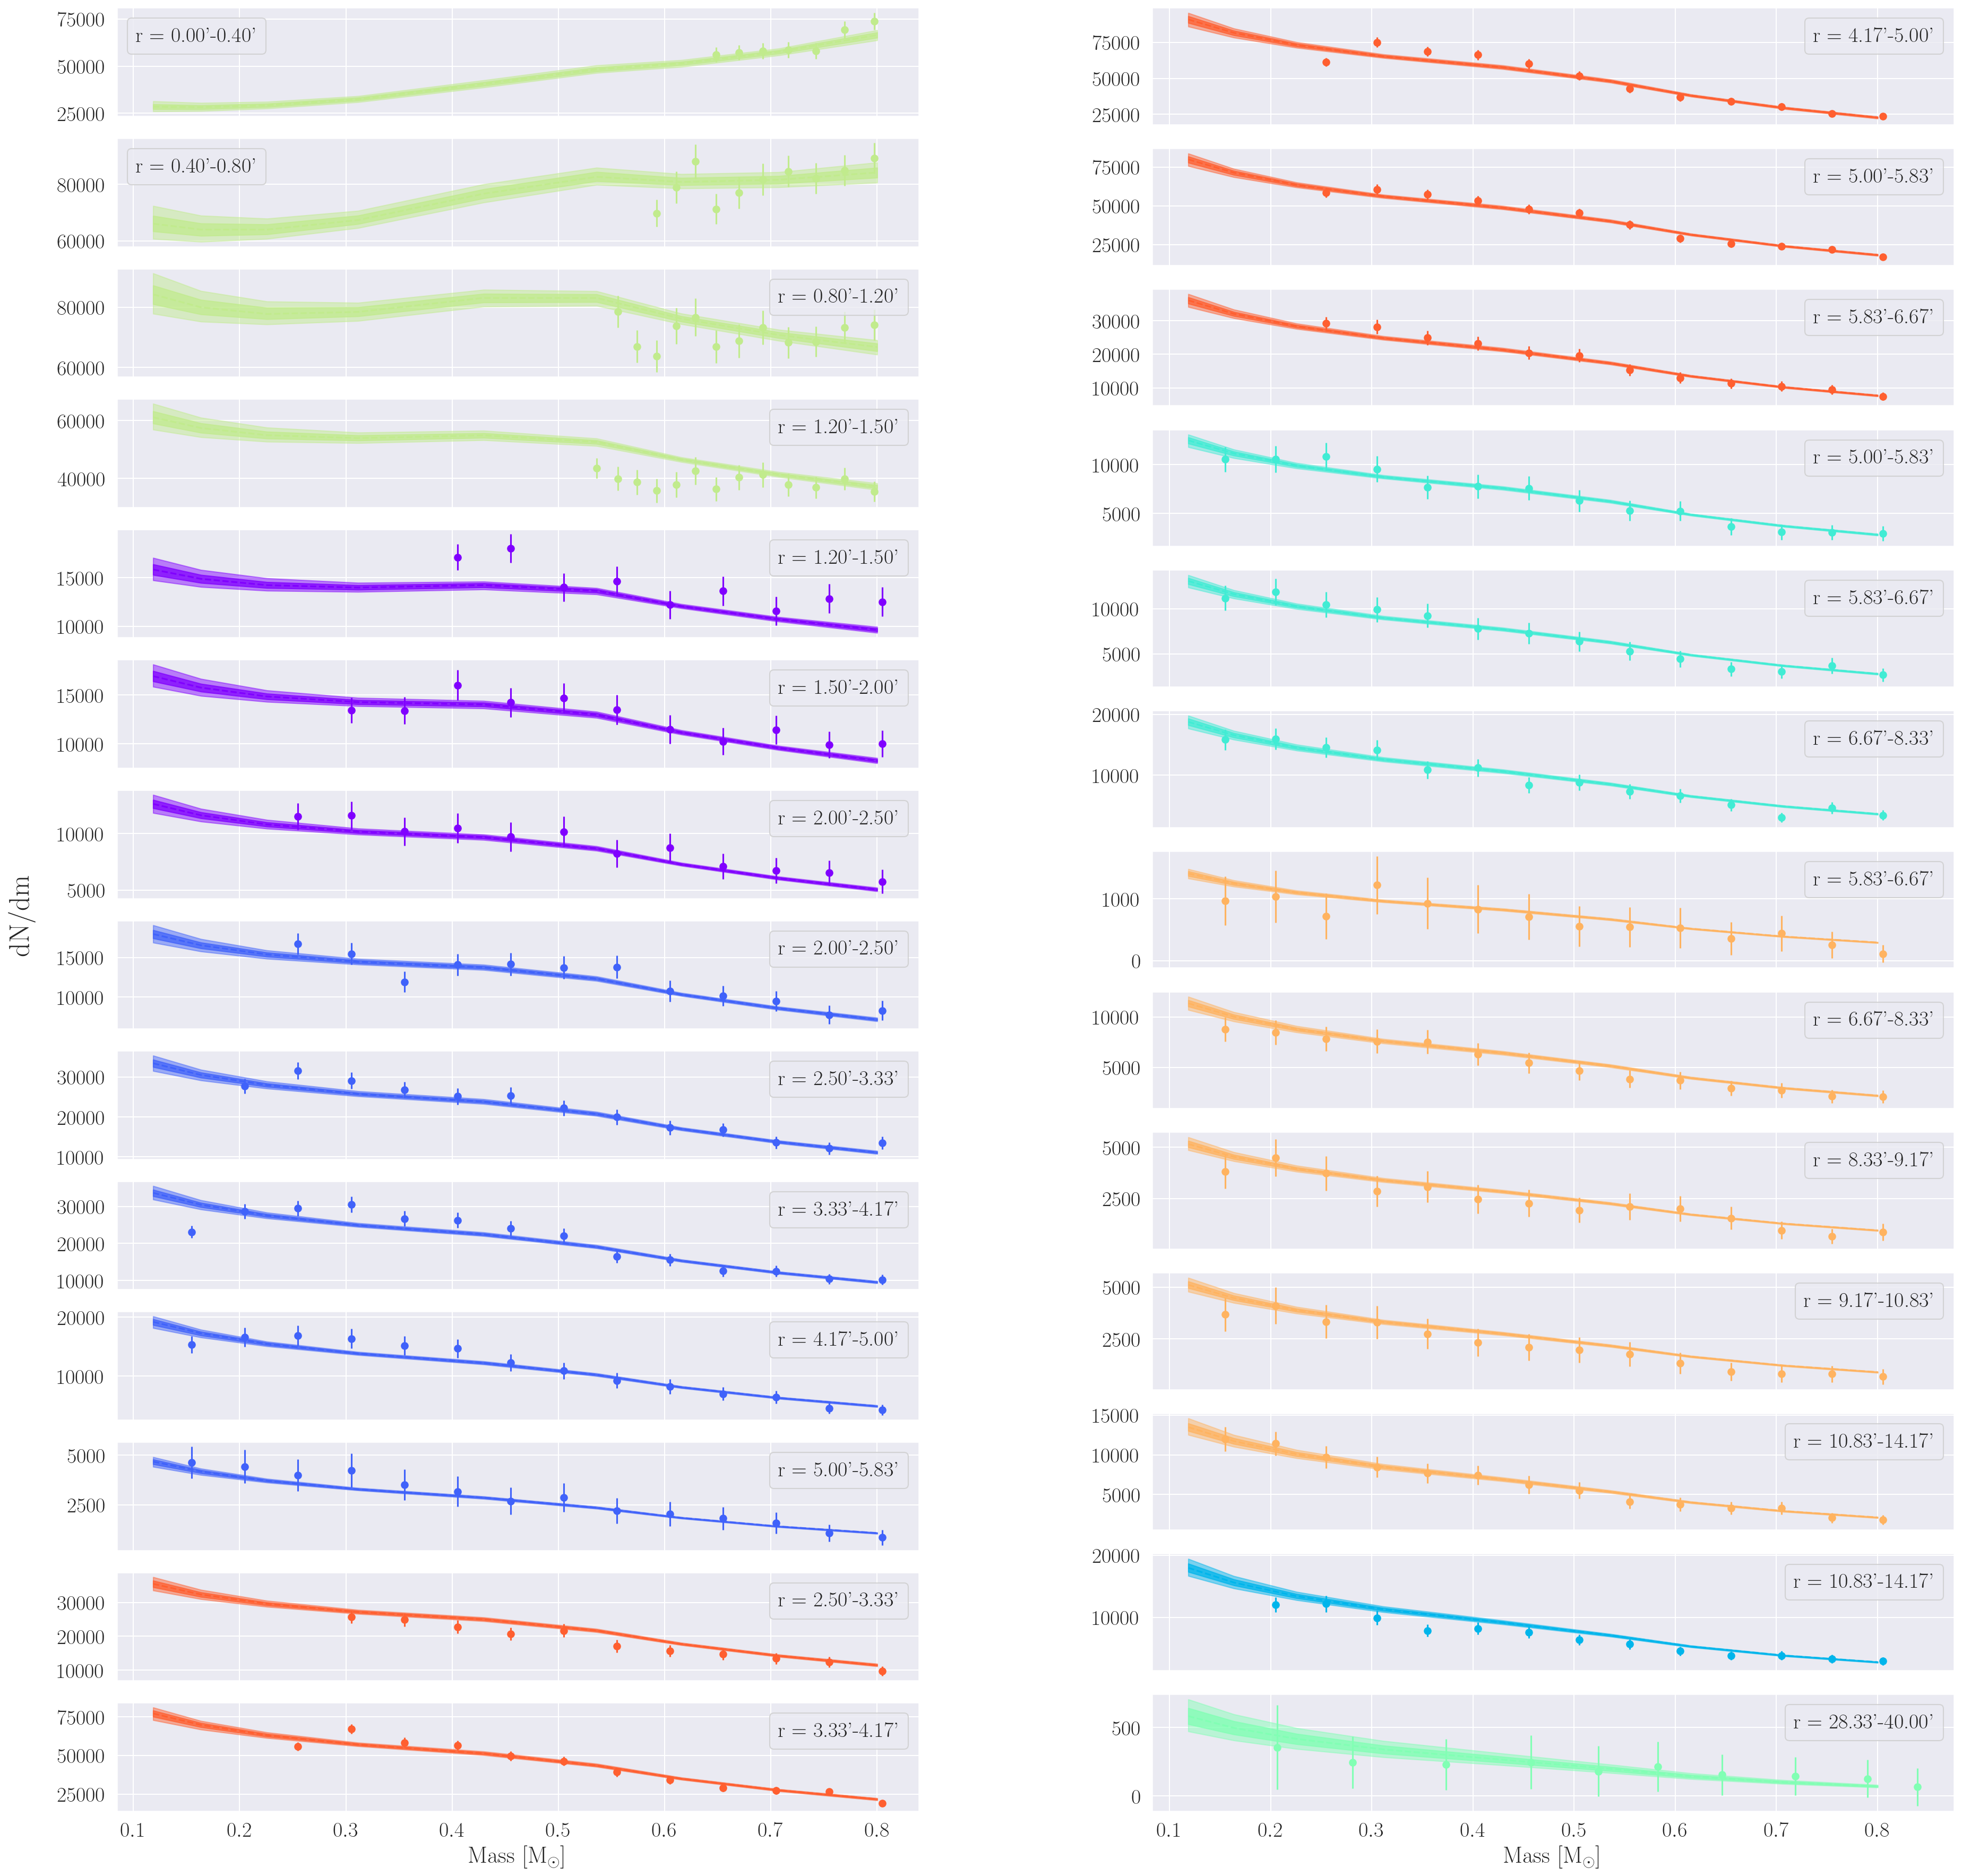
\includegraphics[width=\textwidth]{figures/low_bin_model/mass_fun.png}
	\caption{Model fits to stellar mass function data for models with a $2\%$ binary fraction.}
	\label{fig:low_bin_model_mass_fun}
\end{figure}



\begin{figure}
	\centering
	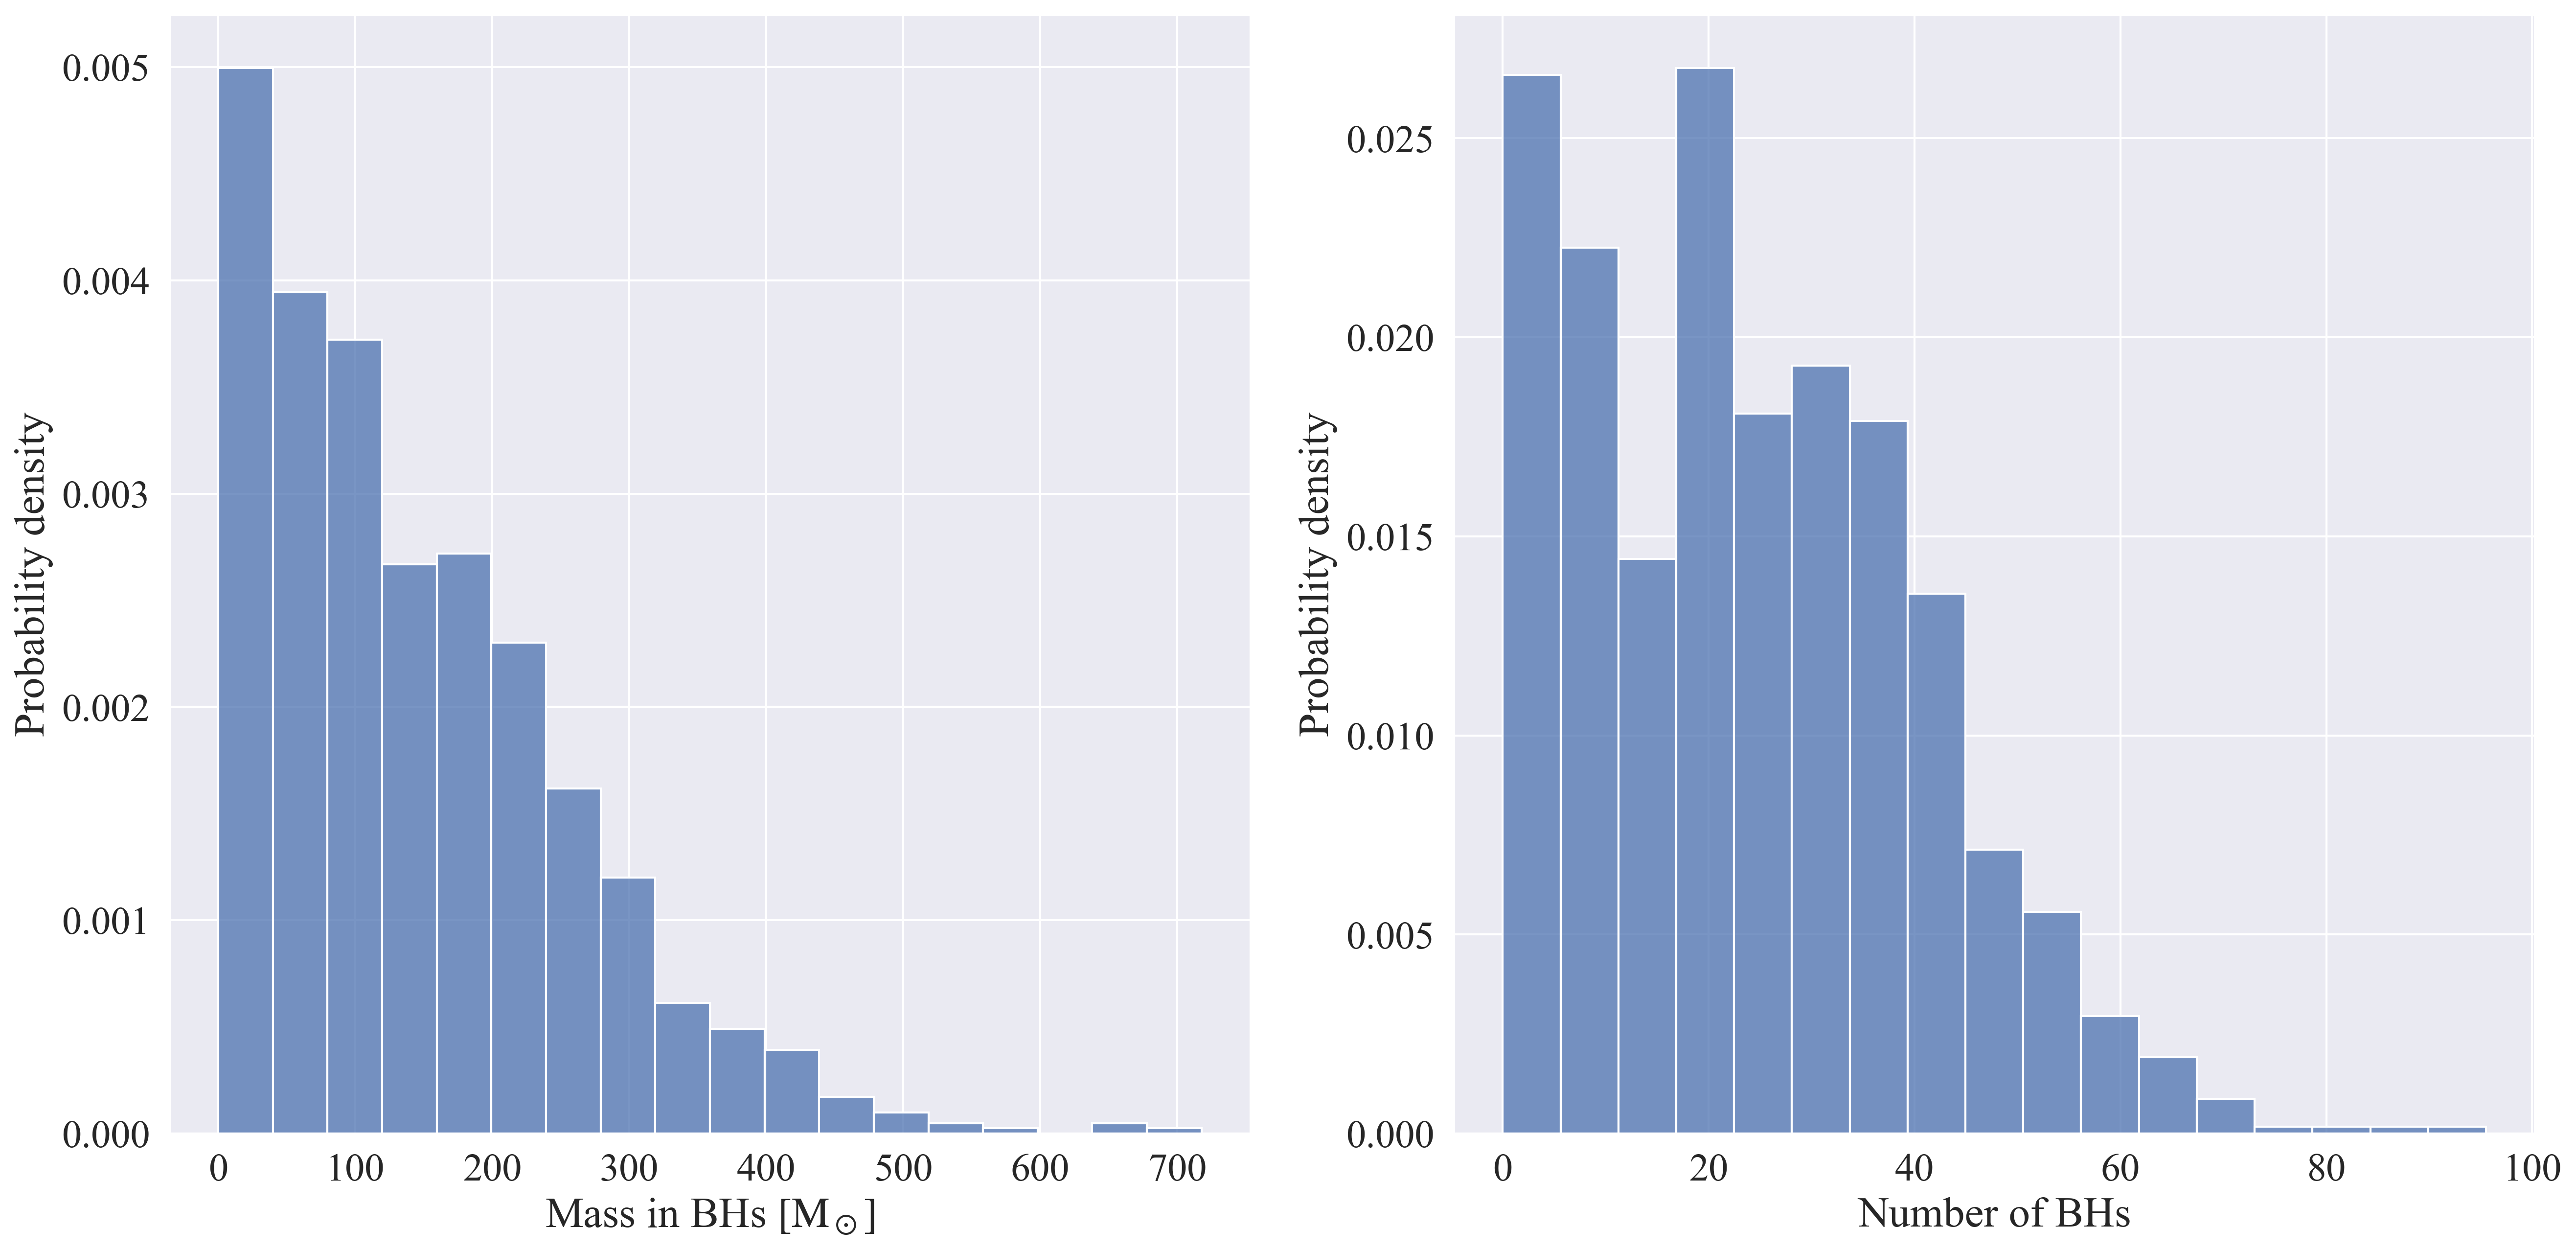
\includegraphics[width=0.8\textwidth]{figures/low_bin_model/BH_dists.png}
	\caption{Distribution in mass and number of black holes for models with a $2\%$ binary fraction.}
	\label{fig:low_bin_model_BH_dists}
\end{figure}


A binary fraction of $2\%$ results in a total mass in binaries of around $15800 \ \mathrm{M}_\odot$,
Figure \ref{fig:low_bin_model_Bin_mass} shows the distribution of mass in binaries in our set of
best-fitting models.


\begin{figure}
	\centering
	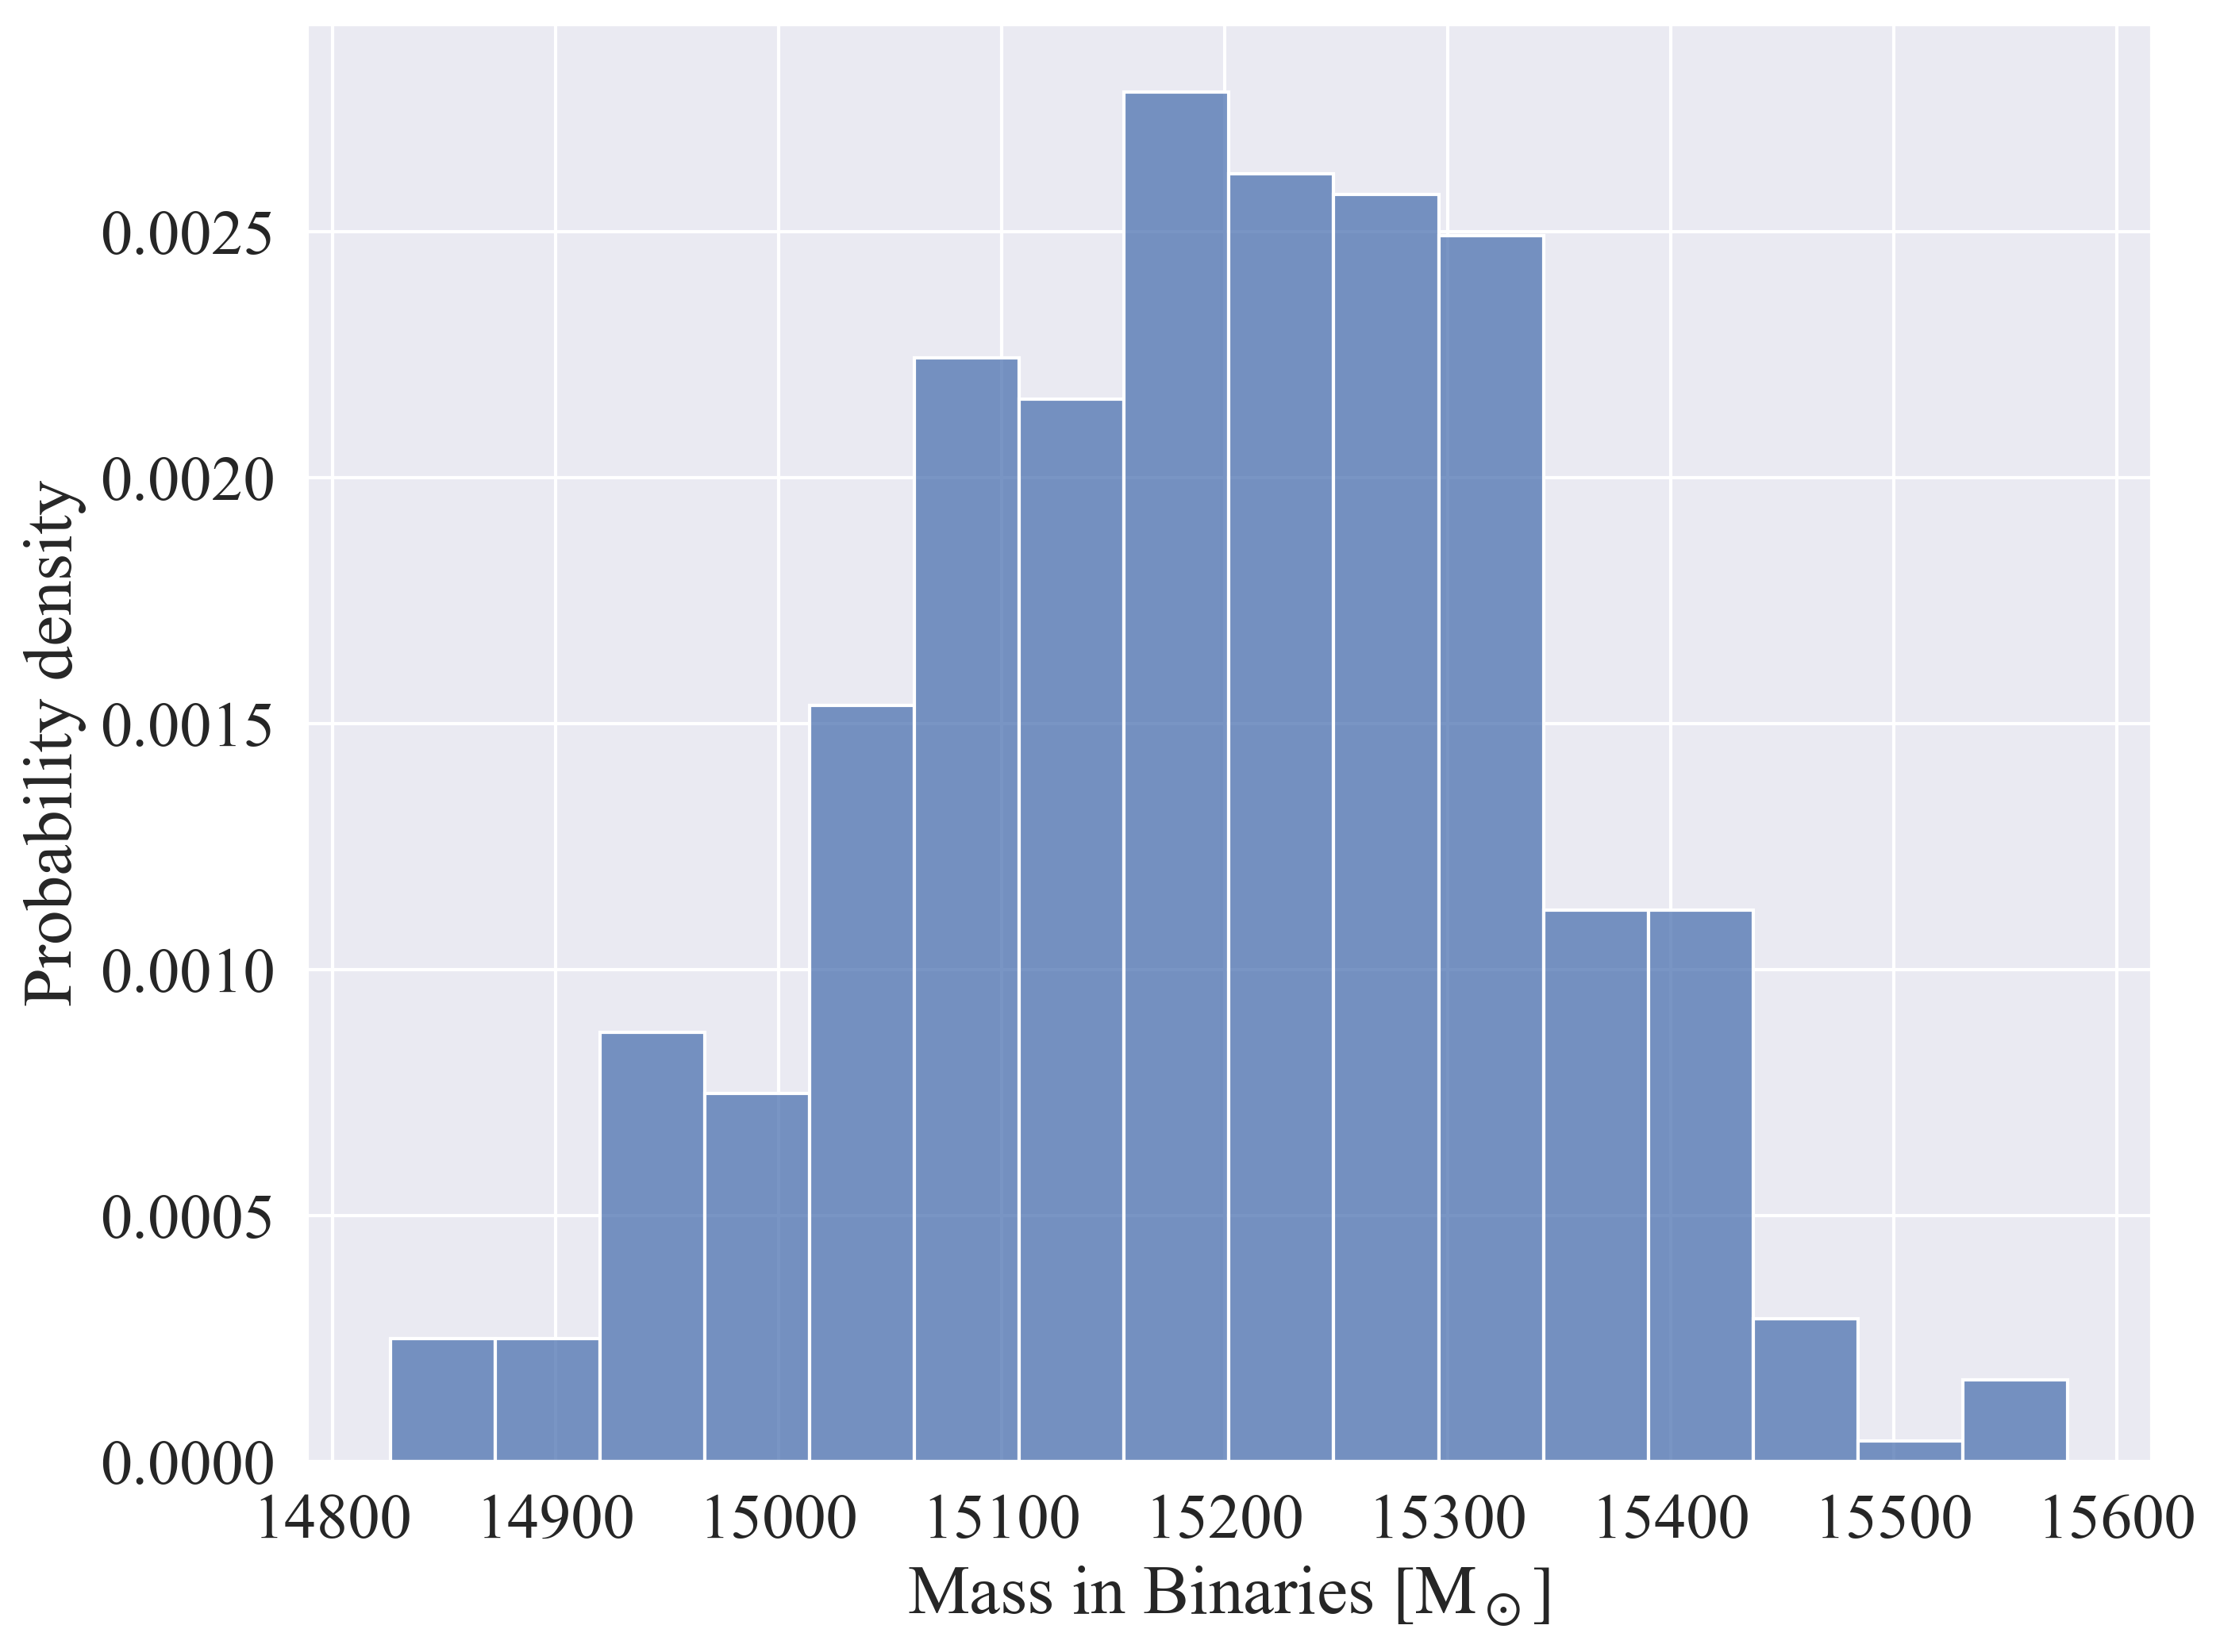
\includegraphics[width=0.8\textwidth]{figures/low_bin_model/binary_mass.png}
	\caption{Distribution of mass in binaries for models with a $2\%$ binary fraction.}
	\label{fig:low_bin_model_Bin_mass}
\end{figure}


\section{High Binary Fraction}

As is the case for the models with a low binary fraction, the models with a $10\%$ binary
fraction fit the observables very well. Figures \ref{fig:highbin_obs_panel} and
\ref{fig:highbin_mass_fun} show the model fits compared to the data.

\begin{table}
	\centering
	\caption{Best-fit parameters with $1\sigma$ credibility intervals for models with a $10\%$ binary fraction.}
	\begin{tabular}{l l}

		\hline
		Parameter                 & Value                  \\
		\hline
		$W_0$                     & $6.36^{+0.09}_{-0.09}$ \\
		$M/10^6 \mathrm{M}_\odot$ & $0.89^{+0.01}_{-0.01}$ \\
		$r_h / pc$                & $6.77^{+0.06}_{-0.06}$ \\
		$\log_{10}{r_a / pc}$     & $1.48^{+0.06}_{-0.05}$ \\
		$g$                       & $1.34^{+0.06}_{-0.06}$ \\
		$\delta$                  & $0.41^{+0.01}_{-0.01}$ \\
		$s^2$                     & $0.01^{+0.01}_{-0.00}$ \\
		$F$                       & $3.16^{+0.13}_{-0.12}$ \\
		$\alpha_1$                & $0.45^{+0.02}_{-0.02}$ \\
		$\alpha_2$                & $1.53^{+0.05}_{-0.04}$ \\
		$\alpha_3$                & $2.46^{+0.05}_{-0.05}$ \\
		$BH_{ret} (\%)$           & $0.17^{+0.18}_{-0.12}$ \\
		$d$                       & $4.43^{+0.02}_{-0.02}$ \\
		\hline
	\end{tabular}
	\label{tab:parameters_highbin}
\end{table}

With a higher binary fraction, we now find fewer black holes, Figure
\ref{fig:high_bin_model_BH_dists} shows the distribution in mass and number which are found to be
$12^{+13}_{-12}$ black holes or $81 ^{+121}_{-81} \ \mathrm{M}_\odot$ in black holes.


\begin{figure}
	\centering
	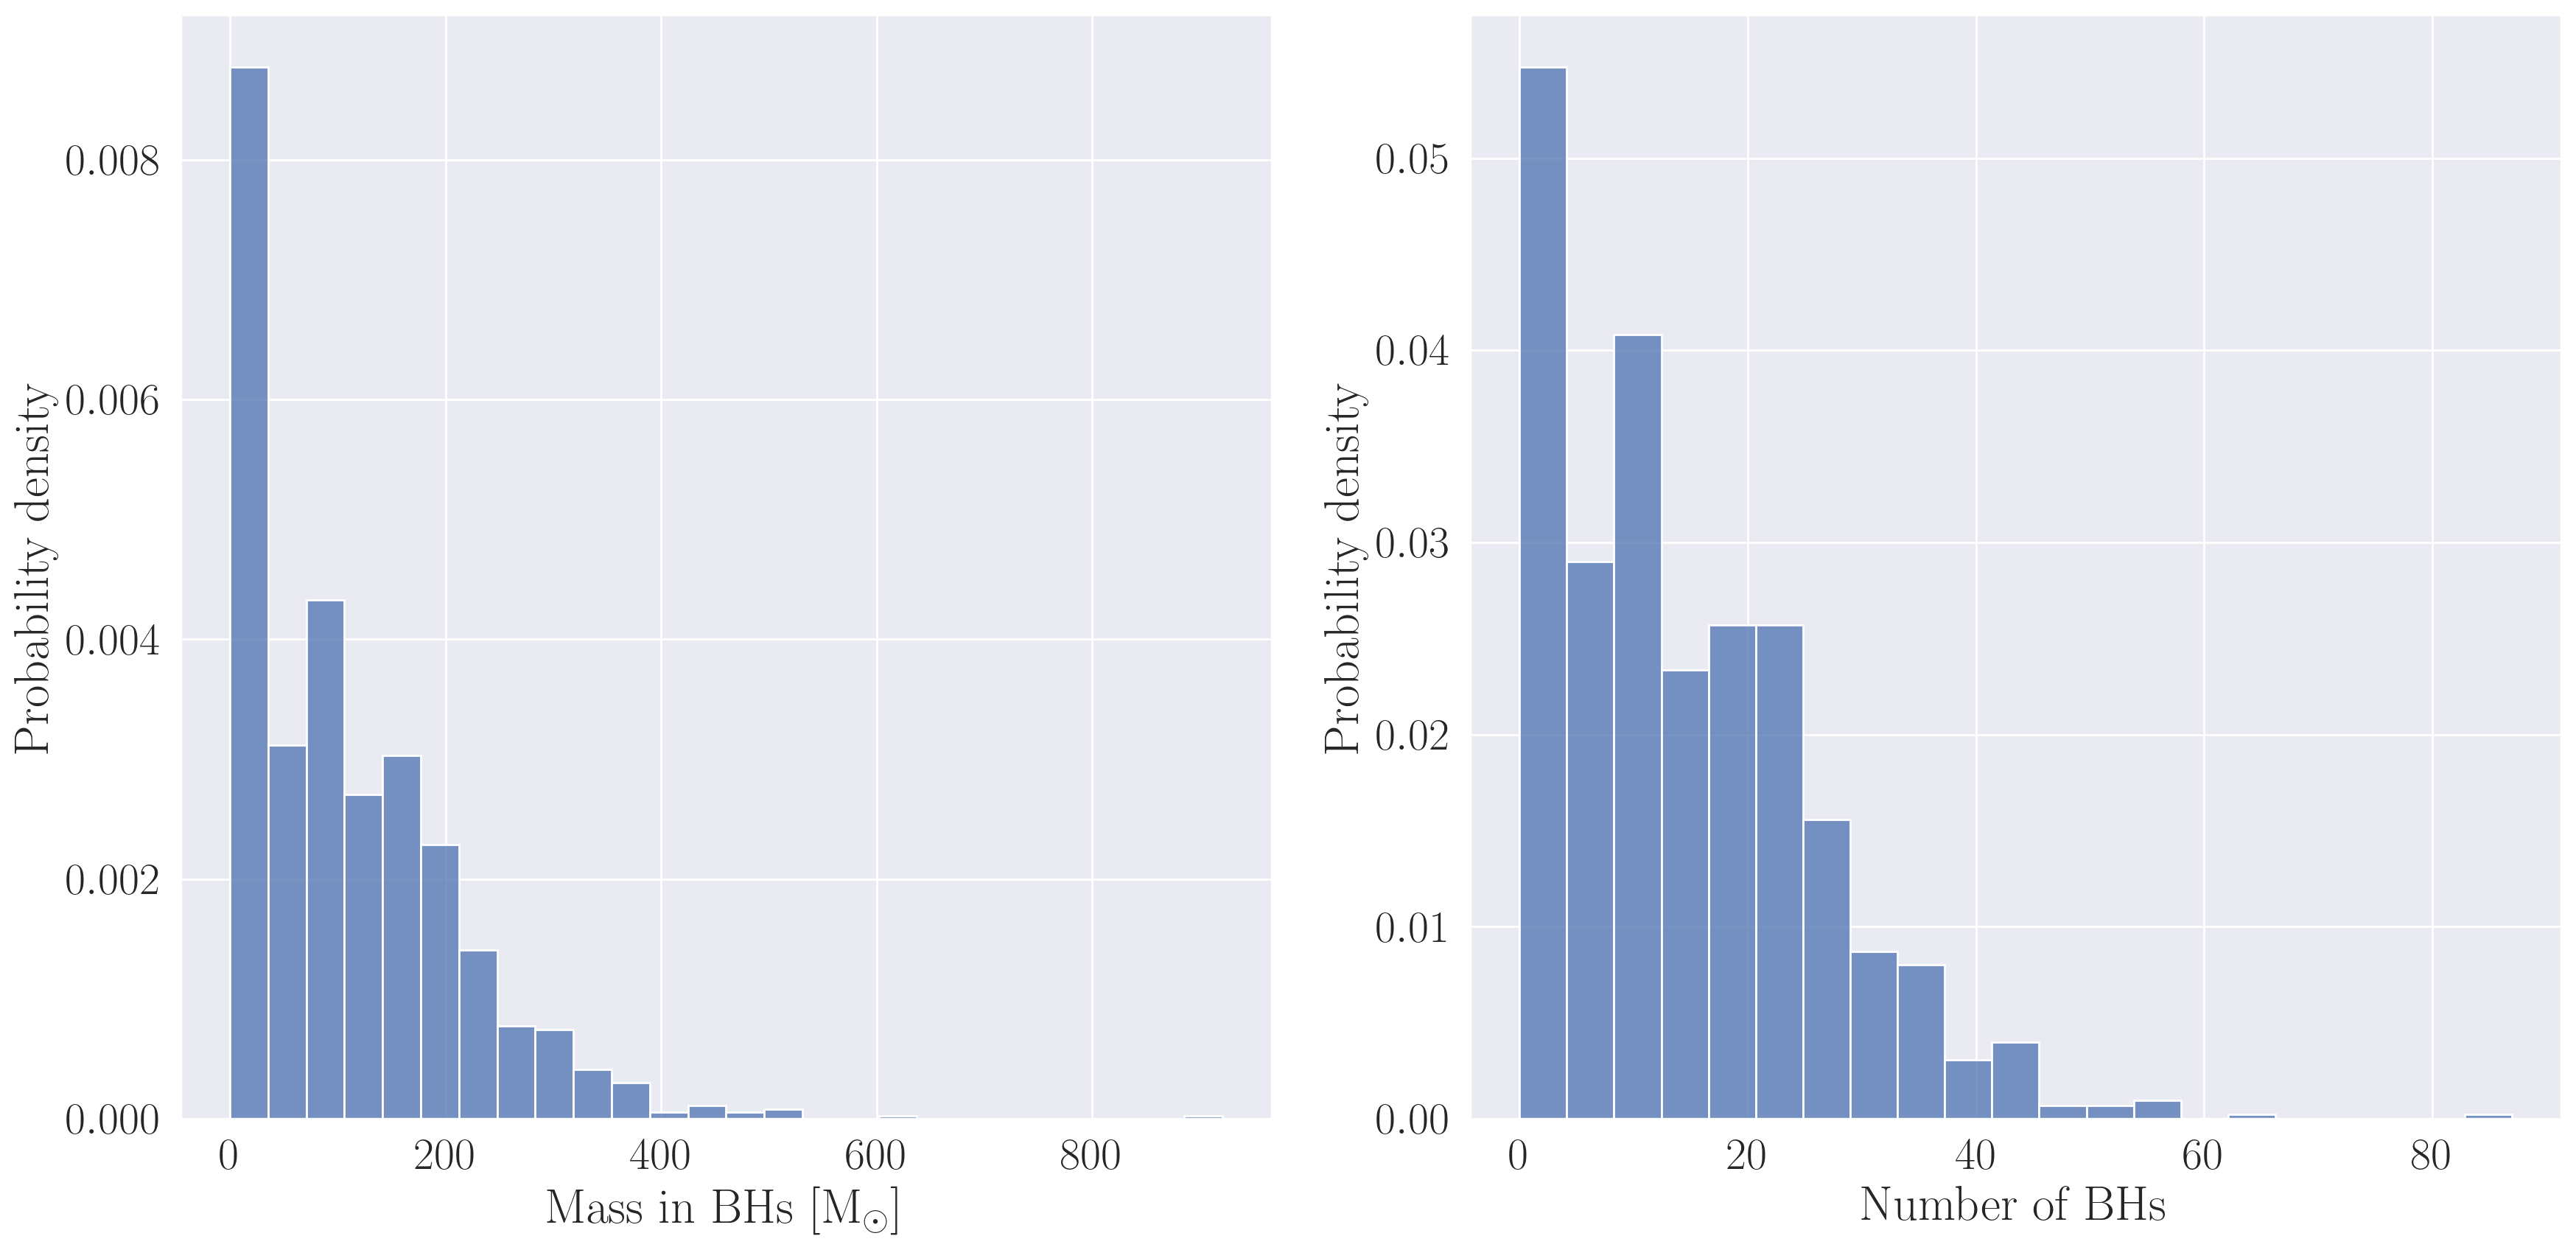
\includegraphics[width=0.8\textwidth]{figures/high_bin_model/BH_dists.png}
	\caption{Distribution in mass and number for models with a $10\%$ binary fraction.}
	\label{fig:high_bin_model_BH_dists}
\end{figure}


With a $10\%$ binary fraction we now have a significant amount of mass in binaries, roughly $81000 \
	\mathrm{M_\odot}$ (see figure \ref{fig:high_bin_model_Bin_mass}), which is a bit less than
$2\%$ of the total cluster mass.

\begin{figure}
	\centering
	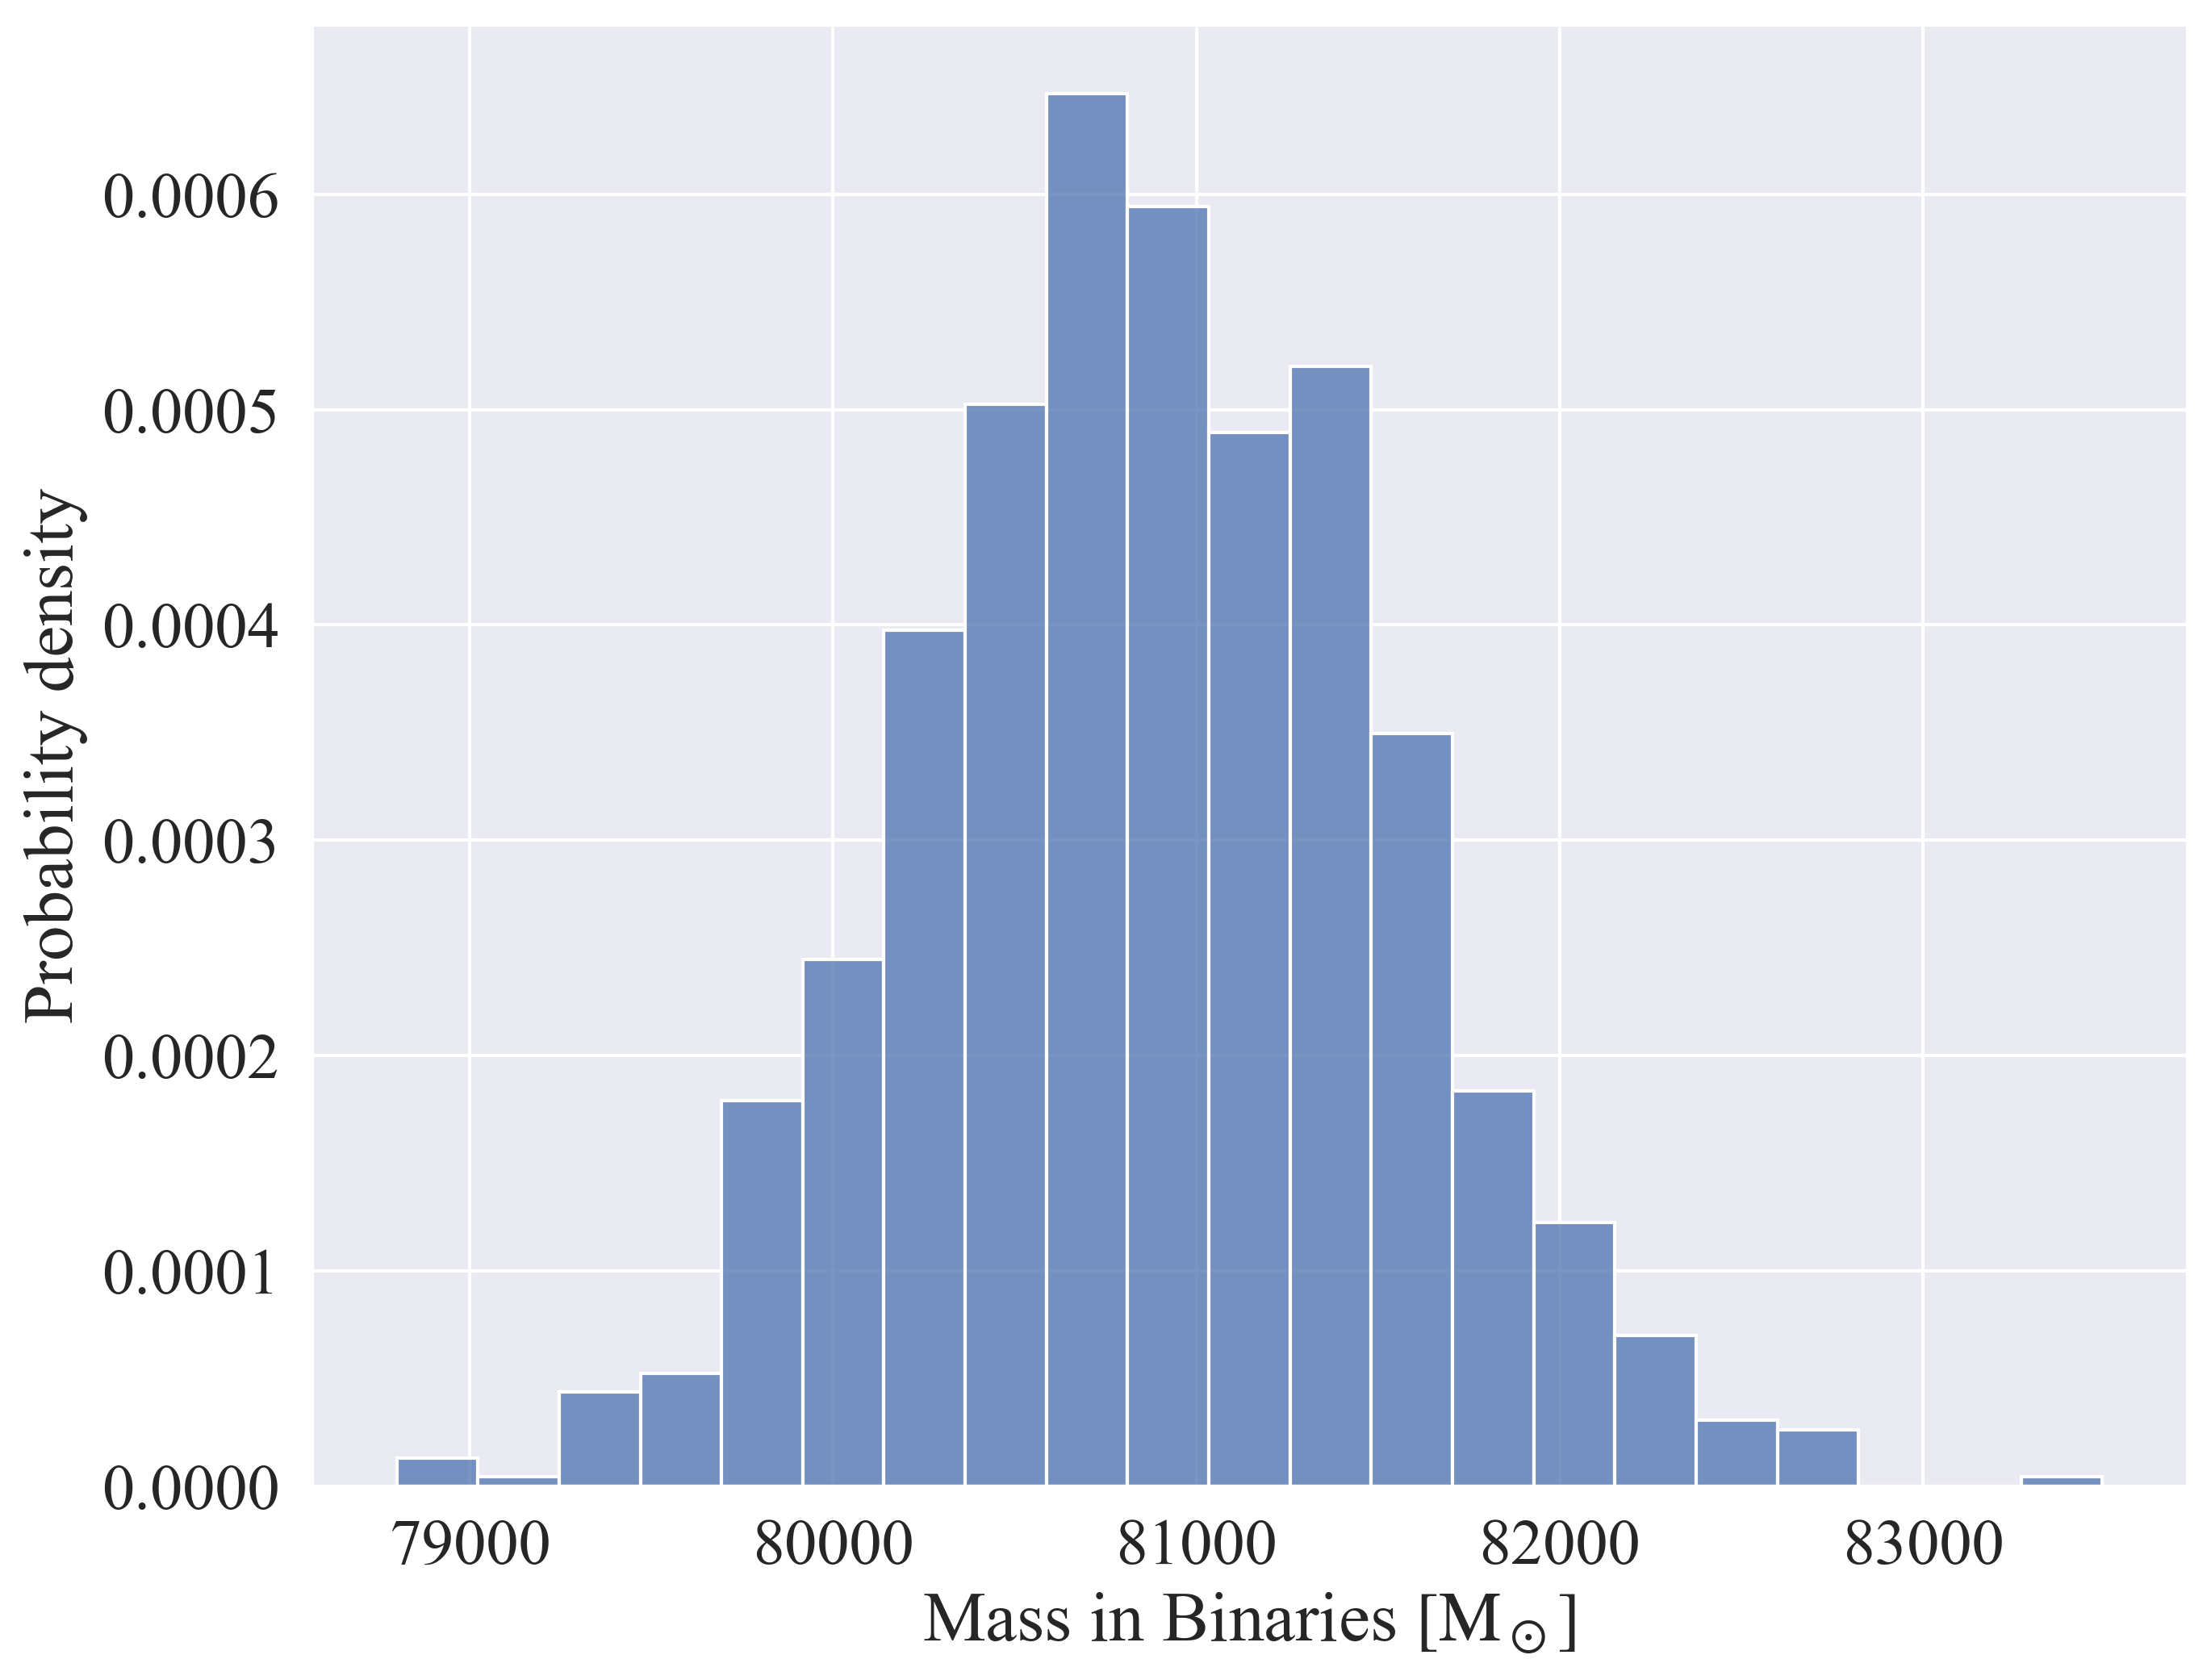
\includegraphics[width=0.8\textwidth]{figures/high_bin_model/binary_mass.png}
	\caption{Distribution of mass in binaries for models with a $10\%$ binary fraction.}
	\label{fig:high_bin_model_Bin_mass}
\end{figure}




